\section{Entwurf}
\label{sec:Entwurf}
Im folgenden Kapitel wird der Entwurf der Anwendung näher beschrieben. Neben den Use Cases und den verwendeten Technologien, wird auch ein Überblick über die System-Architektur gegeben sowie die Kommunikation innerhalb des Systems näher erläutert.

\subsection{Use Cases}
\label{subsec:UseCases}
Aus der Aufgabenstellung ergibt sich eine Reihe von Use Cases, welche in Abbildung~\ref{fig:UseCaseDiagramm} dargestellt sind. 

\begin{figure}[h]
\begin{center}
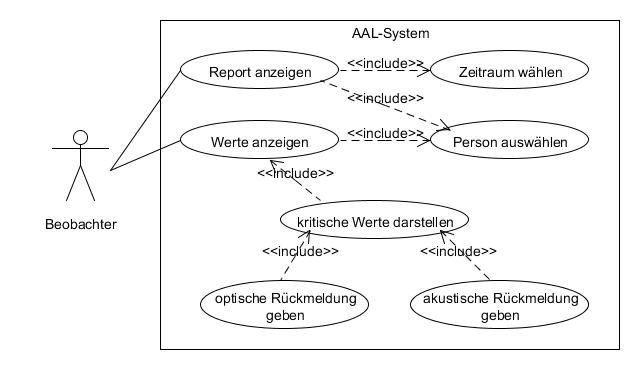
\includegraphics[scale=0.7]{images/AAL-Use-Case-Diagramm.jpg} 
\caption{Use Case Diagramm}
\label{fig:UseCaseDiagramm}
\end{center}
\end{figure}

Der einzige Stakeholder ist ein \textit{Beobachter}. \textit{Beobachter} sind Personen, die die Werte einer Person, zu der Sensorwerte vorliegen, beobachtet. Beispiele für Beobachter sind z.B. Pfleger oder Angehörige. In erste Linie möchte ein \textit{Beobachter}, dass die zu der beobachteten Person passenden Werte angezeigt werden(Use Case:\textit{Werte anzeigen}). Dazu ist es nötig, dass diese Person zuerst ausgewählt wird(Use Case:\textit{Person auswählen}). Um die Werte sinnvoll darzustellen, müssen vor allem kritische Werte gesondert dargestellt werden, da diese meist eine Bedrohung für Leib und Leben der beobachteten Person darstellen. Zu diesem Zweck gibt es zum einen eine optische Rückmeldung(Use Case:\textit{optische Rückmeldung geben}) und zum anderen eine akustische(Use Case:\textit{akustische Rückmeldung geben}).
\\
\\
Neben der zeitnahen Überwachung der Werte soll es ebenfalls möglich sein, eine Zusammenstellung vergangener Werte zu erhalten(Use Case:\textit{Report anzeigen}). Auch dazu muss zuvor die gewünschte Person ausgewählt werden, aber zusätzlich auch ein Datumszeitraum(Use Case:\textit{Zeitraum wählen}). Werden die in diesen Use Cases definierten Grundanforderungen erfüllt, entsteht eine einfache Applikation zur Überwachung von Sensorwerten.


\subsection{Technologien}
\label{subsec:Technologien}
Die folgenden Technologien wurden im Projekt eingesetzt und sollen für das Verständnis näher erläutert werden.

\subsubsection{Node.JS}
\label{subsec:NodeJS}
Node.JS \cite{nodejswebsite} bringt die Programmiersprache Javascript auf die Server-Ebene. Üblicherweise werden Sprachen wie PHP zur Erstellung von Webservices genutzt, um Anwendungen durch Anfragen eines Clients zu starten. Diese Architektur ist jedoch in solchen Fällen ungeeignet, in denen der Client in Echtzeit über Änderungen informiert werden soll. Node.JS ermöglicht es nun Webservices zu erstellen, die mittels Javascript von Anfragen der Clients unabhängig ausgeführt werden können. Hierzu wird die Anwendung beim Start an einen TCP-Port gebunden und erwartet die Anfragen vom Client. Im folgenden Codebeispiel \ref{lst:hellonode} ist gut zu erkennen, dass mit wenig Aufwand ein \textit{"Hello World"}-Server erstellt werden kann.

\begin{lstlisting}
var http = require('http');
http.createServer(function (req, res) {
  res.writeHead(200, {'Content-Type': 'text/plain'});
  res.end('Hello World\n');
}).listen(1337, '127.0.0.1');
console.log('Server running at http://127.0.0.1:1337/');
\end{lstlisting}

Außerdem kann nun aktiv mit dem Client über die geöffnete Verbindung kommuniziert werden. Zum Einsatz kommt dabei die Javascript Engine V8, welche auch im Google Chrome Browser eingesetzt wird. Die besonderen Eigenschaften von Node.JS liegen darin, schnelle und ressourcensparende Webservices zu ermöglichen, die außerdem viele gleichzeitige Anfragen von Clients bewältigen können \cite{cantelon:nodejs}. Dies wird zum einen durch die Auslagerung des I/O-Systems, also den Lese- und Schreiboperationen, in externe Prozesse realisiert. Dadurch werden Abläufe nicht durch die I/O-Operationen blockiert, sondern asynchron verarbeitet. Singlethreading ermöglicht außerdem das Vermeiden von parallelen Zugriffen auf bestimmte Ressourcen, so wie es bei Multithreading der Fall ist. Es müssen sich also keine Gedanken um eventuelle Thread-Safety-Implementierungen gemacht werden. Node.JS bietet ein reichhaltiges Angebot an Zusatzpaketen, die die bestehenden Funktionen erweitern. So ist es möglich z.B. REST-Services oder das Parsen von XML-Dokumenten leicht zu implementieren. Der im Node.JS enthaltene Package Manager (\textit{npm}) lädt alle nötigen Bibliotheken und stellt sie zur Verfügung.

\subsubsection{eXist}
\label{subsec:eXist}
eXist \cite{existwebsite} ist eine in der Sprache Java entwickelte Anwendung, die in ihrer Ursprungsform als eine native XML Datenbank gedacht war \cite{siegel:exist}. Mittlerweile befindet sich das Projekt in der Version 2.2 und umfasst zahlreiche Funktionen, die es ermöglichen, XML-basierte Anwendungen zu erstellen sowie Dokumente in einer NoSQL-Datenbank abzuspeichern und zu verwalten. Die Abfragesprache XQuery\footnote[1]{XML Query Language} ermöglicht das Zugreifen auf die gespeicherten Dokumente. Es können jedoch nicht nur XML-Dokumente in der Datenbank abgelegt werden, sondern nahezu jedes Dateiformat ist erlaubt. So lassen sich eben auch Anwendungen erstellen, die andere Technologien verwenden.
\\
\\
In der stetigen Entwicklung von eXist kam auch eine grafische Oberfläche hinzu, mit der z.B. Code direkt über eine integrierte IDE erstellt und verändert werden kann. Eine Erweiterung des Funktionsumfangs ist durch den Paketmanager leicht möglich. eXist befindet sich weiterhin in der Entwicklung und manche Funktionen sind noch nicht fertig implementiert oder haben noch Fehler. Es ist jedoch in dem jetzigen Stand sehr gut nutzbar.

\subsection{Systemarchitketur}
\label{subsec:Systemarchitketur}
Bei der Systemarchitektur fiel die Wahl auf eine Client-Server Anwendung. Aufgrund der Anforderung, ein Monitoring-System zu erstellen, sprich das der Nutzer über eine grafische Schnittstelle bestimmte Werte angezeigt bekommen lassen möchte, musste ein Client erstellt werden. Weiterhin war gefordert, dass Sensoren von verschiedenen Haushalten aus Daten an das Monitoring-System schicken und diese auch gespeichert werden. Daher musste es eine Möglichkeit geben, die Daten von verschiedenen Quellen in einer zentralen Einheit verwalten zu können. Hierfür wurde ein Server mit integrierter Datenbank ausgewählt. Der erste Entwurf für die Systemarchitektur sah wie folgt aus:

\begin{figure}[h]
\begin{center}
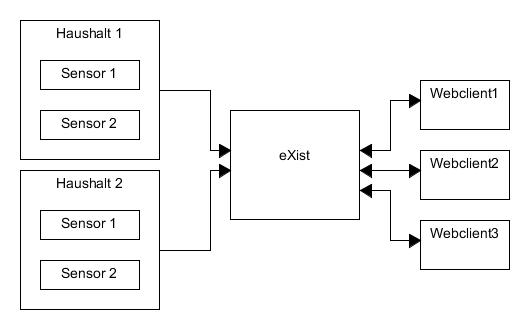
\includegraphics[scale=0.55]{images/sa1.jpg} 
\caption{Erster Entwurf Systemarchitektur}
\end{center}
\end{figure}

\newpage
Ein eXist-Server stellt dabei die zentrale Komponente dar, die sowohl alle Daten von den Sensoren entgegennimmt und verwaltet, sowie auch für die Kommunikation zwischen dem Server und den Clients verantwortlich ist. Für die Sensoren stellt der Server einen REST-Service zur Verfügung, welcher als Übertragungsschnittstelle der ermittelten Vitalwerte dient. So ist es auch leicht möglich, weitere Sensoren an das System anzuschließen, da lediglich die Adresse des REST-Services bekannt sein muss und in welcher Form die Daten übertragen werden müssen. Ansonsten gibt es keine direkte Kopplung. Für die Kommunikation zwischen Server und Clients hätte ebenfalls ein REST-Service verwendet werden können. Hierbei hätte sich jedoch das Problem ergeben, dass sich die Daten von den Sensoren in sehr kurzen Zeitabständen ändern. Um jedoch immer die aktuellsten Vitalwerte anzeigen zu können, müsste der Client sehr oft den Server nach neuen Daten abfragen. Bei mehreren Clients könnte dies zu einer Serverüberlastung führen, da der Server nicht mehr alle Anfragen in kurzer Zeit beantworten kann.
\\
\\
Daher wurde entschieden, die Kommunikation mittels Websockets zu realisieren. Der Vorteil besteht darin, dass der Client nur einmal die Verbindung zum Server aufbaut und dieser dann die Verbindung nutzt, um Daten an den Client zu schicken, ohne dass dieser sich neu verbinden muss. Dies eignet sich besonders gut für das Monitoring-System: Sobald die Sensoren neue Daten schicken, können diese direkt an den wartenden Client weitergeleitet werden, der bereits die Verbindung geöffnet hat und in dem Sinne empfangsbereit für jede Änderung ist. Mit eXist ist eine solche Kommunikationsart nicht möglich, da es keine solche Implementierung der Websockets besitzt. Aus diesem Grund wurde ein zweiter Server hinzugenommen, der sowohl eine REST-Schnittstelle, als auch Websockets zur Verfügung stellt. Die Wahl fiel dabei auf einen Node.JS-Server, da dieser sehr ressourcensparend ist und viele gleichzeitige Netzwerkverbindungen ermöglicht. Der neue Entwurf für die Systemarchitektur ist nun wie folgt:

\begin{figure}[h]
\begin{center}
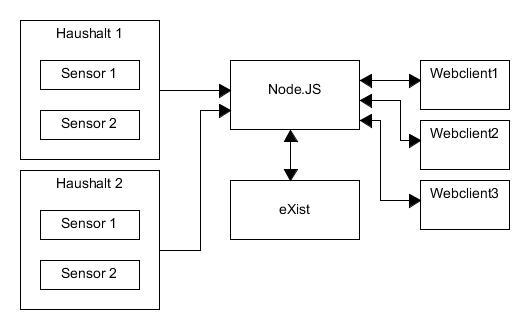
\includegraphics[scale=0.55]{images/sa2.jpg} 
\caption{Zweiter Entwurf Systemarchitektur}
\end{center}
\end{figure}

Der Node.JS-Server ist die zentrale Einheit und steuert die Kommunikation zwischen den Sensoren und den Clients. Weiterhin speichert er alle empfangenen Werte in der eXist-Datenbank ab. Hauptsächlich besteht die Aufgabe des Node.JS-Servers darin, die Anfragen und Antworten an die entsprechenden Stellen (eXist, Client) weiterzuleiten. Dies war jedoch nötig, um sowohl REST-Services, als auch Websockets verwenden zu können.

\subsection{Kommunikation}
\label{subsec:Kommunikation}
Die Sensoren schicken ihre ermittelten Werte (\textit{sensorData}) an den Node.JS -Server. Dabei wird die Antwort von den Sensoren jedoch ignoriert, da auf dieser Seite keine  Fehlerbearbeitung vorgesehen ist. Die Daten werden über eine REST-Anfrage (POST) mit dem entsprechenden XML-Dokument gesendet.

\begin{figure}[H]
\begin{center}
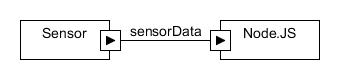
\includegraphics[scale=0.6]{images/komm1.jpg} 
\caption{Kommunikation zwischen Sensoren und Node.JS-Server}
\end{center}
\end{figure}

\newpage
Der eXist-Server bietet zur Kommunikation einen Standard, mit dem sich mittels XQuery REST-Services erstellen lassen. \textit{RESTXQ} bietet verschiedene Annotationen, um beispielsweise einen URL-Pfad anzugeben, unter dem eine Funktion von außerhalb angesprochen werden kann, oder um die Funktion als eine POST-Methode festzulegen. Mit Hilfe der Annotationen wurde nun die Kommunikation zwischen dem Node.JS-Server und der eXist-Datenbank hergestellt. Die von den Sensoren empfangenen Daten werden mittels POST an die Datenbank geschickt (\textit{sensorData}). Weiterhin kann mittels einem \textit{reportRequest} ein Report für eine bestimmte Person in einem Zeitraum über alle Vitalwerte angefordert werden. Der eXist sendet daraufhin die erstellte PDF-Datei als \textit{reportData} wieder zum Node.JS-Server. Außerdem kann geprüft werden, ob eine \textit{personId} in der Datenbank bereits verzeichnet ist. Dafür sendet der Node.JS-Server eine Anfrage mit der \textit{personId} an eXist und erhält eine Meldung über die Existenz der ID (\textit{personIdResponse}).

\begin{figure}[h]
\begin{center}
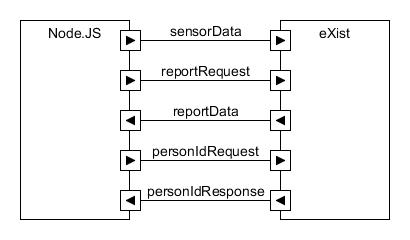
\includegraphics[scale=0.6]{images/komm2.jpg} 
\caption{Kommunikation zwischen Node.JS-Server und eXist}
\end{center}
\end{figure}

Von den Clients aus können sowohl die Reports, als auch die Überprüfung der gewünschten \textit{personId} angefordert werden. Der Node.JS-Server leitet diese Anfragen an eXist weiter und gibt die Antworten an die Clients zurück. Diese Anfragen hätten auch über einen REST-Service erstellt werden können, man entschied sich aber dafür, die Kommunikationsarten auf Clientseite nicht zu vermischen. Außerdem erhält der Client über die offene Websocket-Verbindung jeden neuen Wert, der von den Sensoren geschickt wurde.  \\ \\

\begin{figure}[h]
\begin{center}
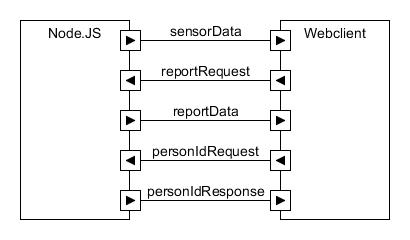
\includegraphics[scale=0.6]{images/komm3.jpg} 
\caption{Kommunikation zwischen Node.JS-Server und Client}
\end{center}
\end{figure}

\newpage
Zur Übermittlung der Daten von den Sensoren zum Server wurde eine XML-Struktur verwendet, welche in Abbildung~\ref{lst:sensorXml} zu sehen ist. Die \texttt{personId} identifiziert die Person, der der gesendete Datensatz zugeordnet wird. Die \texttt{roomId} symbolisiert den Aufenthaltsort der Person, wobei der Wert auch eine Abstrakte Id sein kann und keine physische Lokalität. Der \texttt{timestamp} beinhaltet die Uhrzeit und das Datum der Erfassung des Datensatzes. Das gewählte Format richtet sich dabei nach der Speicherung im eXist, um die Verarbeitung zu erleichtern. Der \texttt{sensor} Tag beinhaltet den Typ (\texttt{type}) des Sensors und seinen Wert(\texttt{value}). Durch die separate Angabe des Typs als Textwert in der XML ist es leicht möglich, diese XML-Struktur für weitere Sensortypen zu verwenden. Ebenso kann der Wert sehr allgemein geschickt werden, z.B. auch als String mit physikalischer Einheit. Der \texttt{status} kann genutzt werden um direkt zu übermitteln, ob ein Wert in einem kritischen Bereich liegt. Dadurch ist es nicht nötig, dass der Empfänger Kenntnis von den Grenzwerten hat.

\begin{lstlisting}[caption={SensorXML},label=lst:sensorXml]
<sensorData>
   <personId>Andre</personId>
   <roomId>Wohnzimmer</roomId>
   <timestamp>
      <time>15:33:58 PM</time>
      <date>2015-06-24</date>
   </timestamp>
   <sensor>
      <type>Herzschlag</type>
      <value>120</value>
      <status>normal</status>
   </sensor>
</sensorData>
\end{lstlisting}